\clearpage
\appendix
% Identificar os apêndices também no cabeçalho e nas referências cruzadas.
\renewcommand{\thesection}{\appendixname~\Alph{section}}
\renewcommand{\thesubsection}{\Alph{section}.\arabic{subsection}}
\titleformat{\section}[block]{\normalfont\normalsize\bfseries\filcenter}{\thesection\space---}{\fontdimen2\font}{}
\section{Painéis completos de energia e construção}
\label{anexo:paineis}

\begin{figure}[!ht]
\centering
\caption{Energia (3500): todas as sete entradas e as saídas 1--31 de 62.}
\label{fig:anexo-energia}
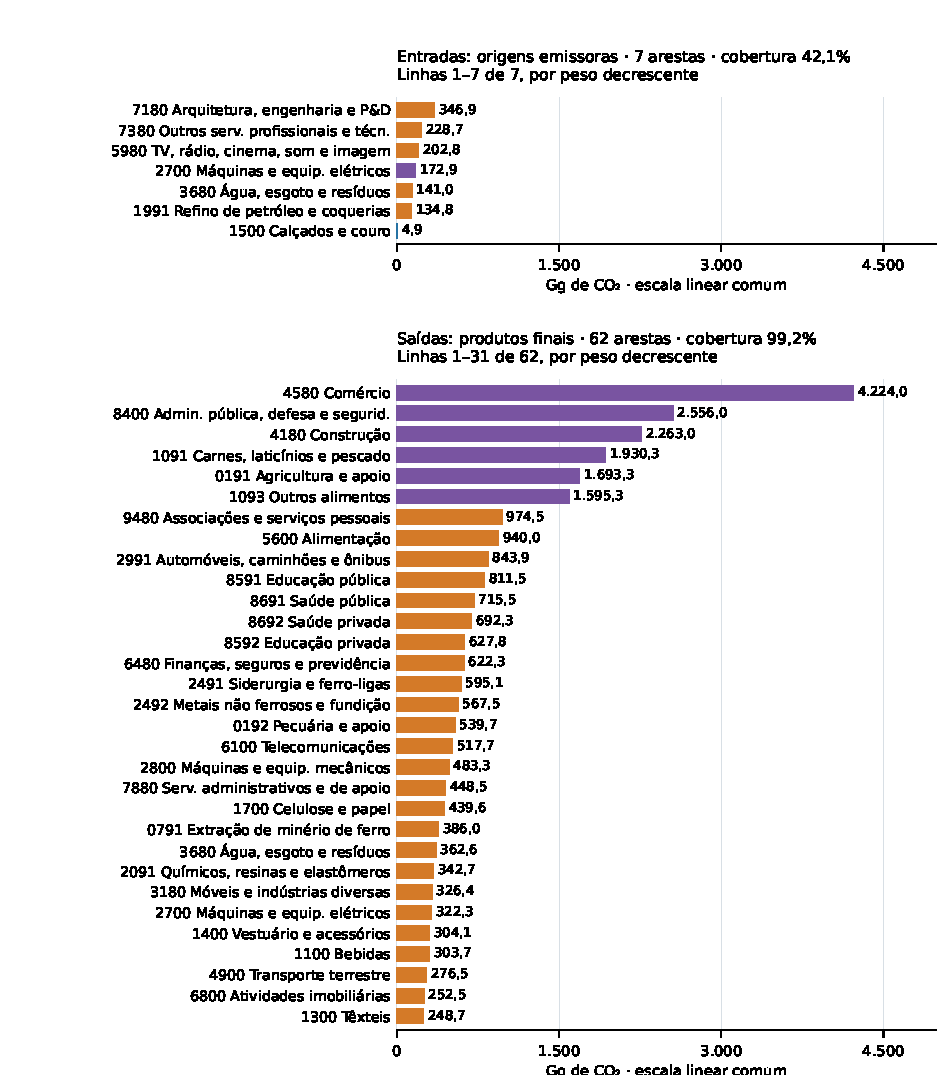
\includegraphics[width=\textwidth,height=0.78\textheight,keepaspectratio]{figuras/anexo_energia_1.pdf}
\begin{notas}
Nota: Recortes de $\alpha=0{,}05$, com pesos originais em Gg de CO\textsubscript{2}, uma casa decimal e escala linear comum. A cobertura é o peso retido sobre a força da atividade e direção em $W$, sem diagonal: 42,1\% nas entradas e 99,2\% nas 62 saídas. As demais saídas aparecem na continuação, sem novo filtro. Azul: só saída na origem; laranja: só entrada no destino; roxo: ambos os testes.
\end{notas}
\end{figure}
\clearpage
\begin{figure}[p]
\ContinuedFloat
\centering
\caption{Energia (3500), continuação: saídas 32--62 de 62.}
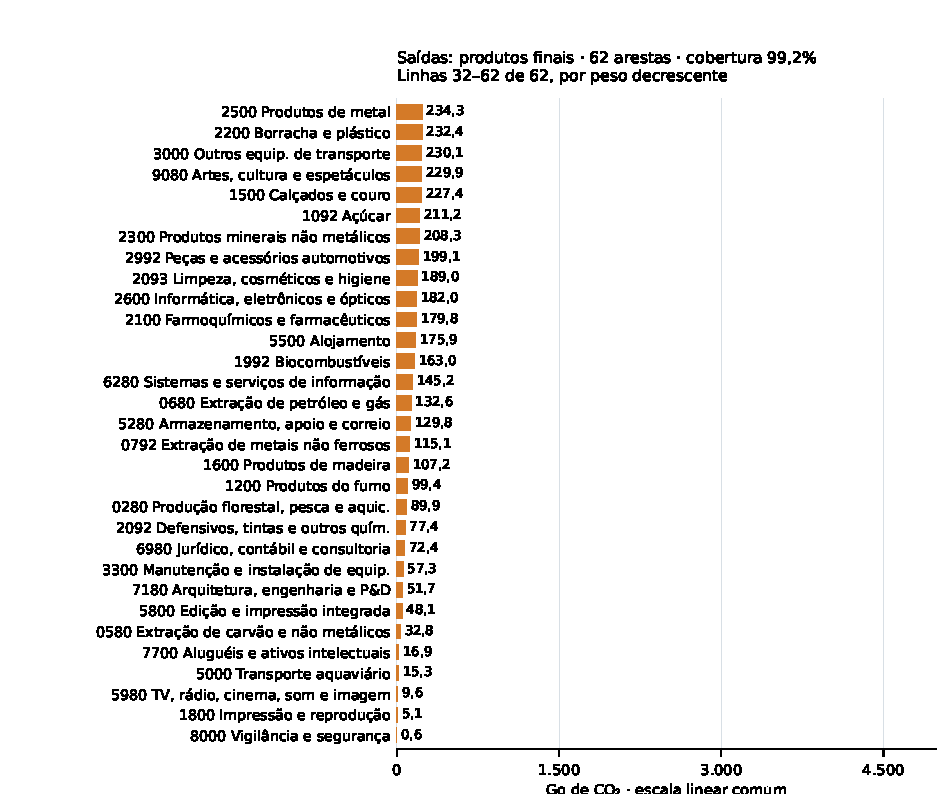
\includegraphics[width=\textwidth,height=0.85\textheight,keepaspectratio]{figuras/anexo_energia_2.pdf}
\begin{notas}
Nota: Mesma seleção, ordem, escala e cores do painel anterior. A cobertura de 99,2\% se refere às 62 saídas, não apenas a esta página. Azul: só saída na origem; laranja: só entrada no destino; roxo: ambos os testes.
\end{notas}
\end{figure}
\clearpage
\begin{figure}[p]
\centering
\caption{Construção (4180): todas as 45 entradas e cinco saídas.}
\label{fig:anexo-construcao}
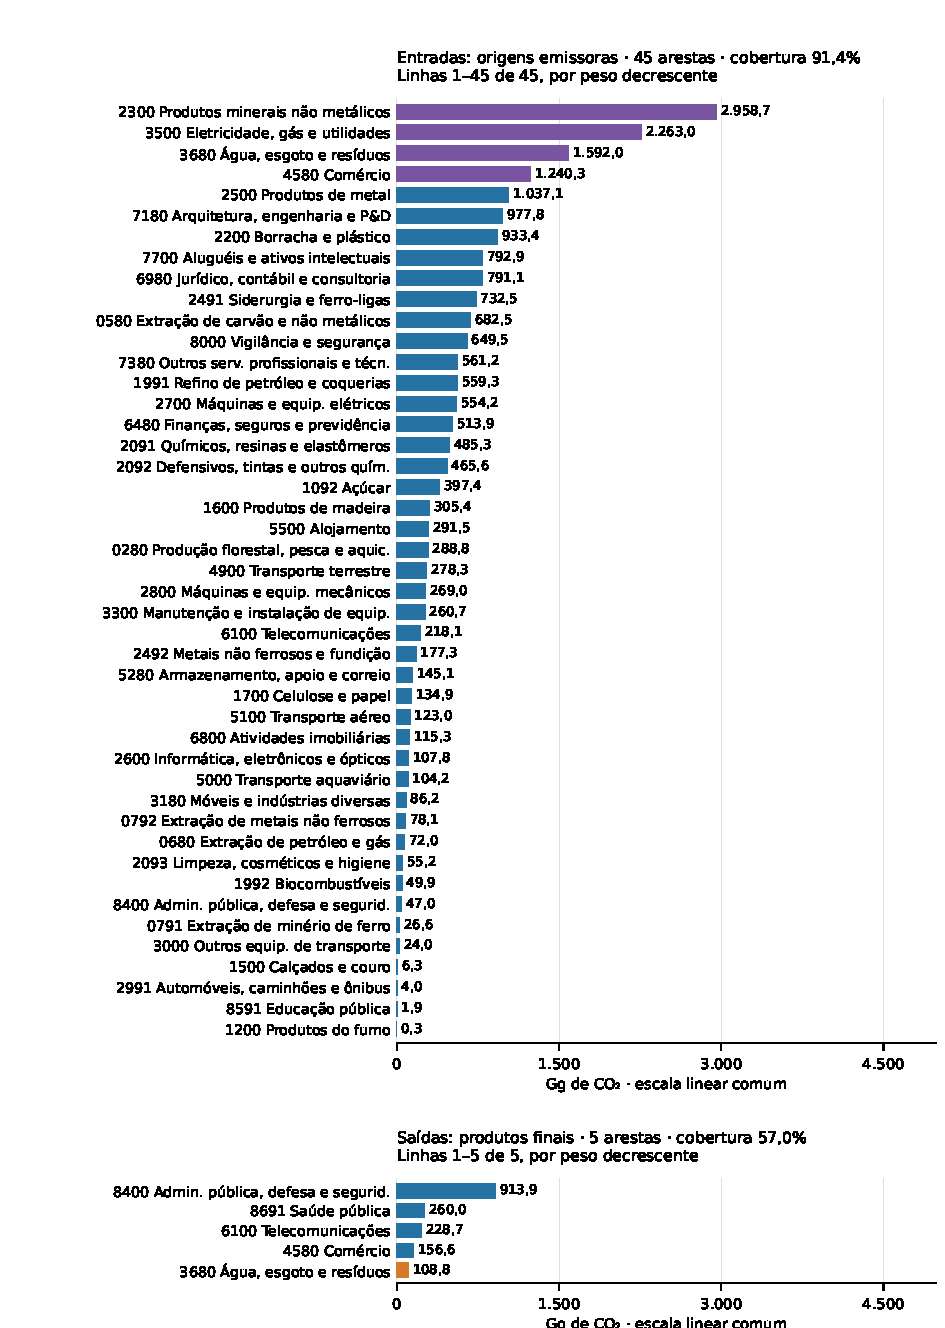
\includegraphics[width=\textwidth,height=0.85\textheight,keepaspectratio]{figuras/anexo_construcao.pdf}
\begin{notas}
Nota: Coberturas de 91,4\% nas entradas e 57,0\% nas saídas. Mesma escala de pesos dos painéis de energia. Azul: só saída na origem; laranja: só entrada no destino; roxo: ambos os testes. Arestas compartilhadas não são duplicadas na rede.
\end{notas}
\end{figure}
\clearpage

\section{Diagnósticos complementares da rede e da seleção}
\label{anexo:diagnosticos}

Na rede completa, os 66 perfis definidos têm medianas de 11,50 destinos efetivos e 13,93 origens efetivas, abaixo das 65 contrapartes existentes em cada direção. No backbone com $\alpha=0{,}05$, as medianas de cobertura são 59,32\% nas saídas e 55,69\% nas entradas.

A Tabela~\ref{tab:postos-complementares} detalha as mudanças de posição por grau em relação a $\alpha=0{,}05$. Os postos são calculados em ordem decrescente entre os 67 nós, com posto médio nos empates; reporta-se a mediana da mudança absoluta.

\begin{table}[htbp]
\centering
\caption{Mudança mediana de posição por grau em relação a $\alpha=0{,}05$.}
\label{tab:postos-complementares}
\begin{tabular}{@{}crr@{}}
\toprule
$\alpha$ & Grau de saída & Grau de entrada \\
\midrule
0,01 & 11 & 7 \\
0,10 & 4,5 & 4 \\
\bottomrule
\end{tabular}
\begin{notas}
Nota: Valores em posições; as diferenças são calculadas a partir dos postos não arredondados, incluindo empates.
\end{notas}
\end{table}

Dos 575 vínculos retidos em $\alpha=0{,}05$, 232 passam somente pelo teste de saída na origem, 265 somente pelo de entrada no destino e 78 pelos dois. Nenhum depende da convenção de grau um. A seleção por apenas uma extremidade mostra que uma relação pode destacar-se em um perfil sem ter a mesma importância relativa no outro.

Nos recortes da Tabela~\ref{tab:motivos-casos}, o backbone omite 57,9\% das entradas externas de energia e 43,0\% das saídas externas de construção. Esses complementos das coberturas evidenciam o volume omitido nas direções com menos ligações selecionadas.


\subsection{Sensibilidade dos perfis focais}

A Tabela~\ref{tab:sensibilidade-casos} acompanha os mesmos cinco perfis completos nos três parâmetros. A última coluna conta quantas das cinco maiores contrapartes de $W$ permanecem em cada backbone; a cobertura usa o volume completo da atividade e direção. A verificação da permanência é distinta da estabilidade dos pesos: as contas, os pesos e os números efetivos de $W$ são os mesmos em todos os parâmetros.

\begin{table}[htbp]
\centering
\caption{Sensibilidade das ligações e da cobertura nos perfis focais.}
\label{tab:sensibilidade-casos}
\small
\begin{tabular}{@{}lcrrr@{}}
\toprule
Perfil & $\alpha$ & Arestas & Cobertura (\%) & Das cinco maiores \\
\midrule
Energia: saídas & 0,01 & 54 & 92,12 & 5 \\
 & 0,05 & 62 & 99,23 & 5 \\
 & 0,10 & 64 & 99,96 & 5 \\
\addlinespace
Água/resíduos: saídas & 0,01 & 29 & 74,85 & 4 \\
 & 0,05 & 49 & 92,98 & 5 \\
 & 0,10 & 57 & 97,24 & 5 \\
\addlinespace
Construção: entradas & 0,01 & 32 & 74,31 & 4 \\
 & 0,05 & 45 & 91,38 & 5 \\
 & 0,10 & 55 & 97,76 & 5 \\
\addlinespace
Energia: entradas & 0,01 & 4 & 25,77 & 3 \\
 & 0,05 & 7 & 42,14 & 5 \\
 & 0,10 & 12 & 61,94 & 5 \\
\addlinespace
Construção: saídas & 0,01 & 4 & 51,61 & 4 \\
 & 0,05 & 5 & 56,96 & 5 \\
 & 0,10 & 7 & 64,29 & 5 \\
\bottomrule
\end{tabular}
\begin{notas}
Nota: Cada perfil tem 65 ligações em $W$. A última coluna varia de zero a cinco e registra a presença das principais contrapartes, independentemente da extremidade responsável pela seleção. Água/resíduos $\rightarrow$ construção, terceira maior origem externa da construção e quinto maior destino de água/resíduos, não é retida em $\alpha=0{,}01$. Energia $\rightarrow$ construção permanece pelos dois testes nos três parâmetros. A sensibilidade não mede a incerteza dos coeficientes ambientais.
\end{notas}
\end{table}
